\documentclass[11pt, a4paper]{article}
%-----------------------
%- 	PACKAGES & SETTINGS
%-----------------------
\usepackage[a4paper,top=2cm,bottom=2cm,left=2cm,right=2cm]{geometry}
\renewcommand{\baselinestretch}{1} 
\usepackage[utf8]{inputenc}
\usepackage[T1]{fontenc}
\usepackage[italian]{babel}
\usepackage{xcolor}
\usepackage{tabto}
\usepackage{hyperref}
\hypersetup{
    colorlinks=true,
    filecolor=magenta,      
    urlcolor=darkgray,
    linkcolor=black
}
\urlstyle{same}
\usepackage{amsmath}
\usepackage{subfloat}
\usepackage{graphicx}
\graphicspath{ {images/} }
 
\begin{document}
%-----------------------
%- 	TITLE
%-----------------------
\begin{titlepage}
    \begin{center}
        \vspace*{1cm}
            
        \Huge
        \textbf{Relazione Progetto}
            
        \vspace{0.5cm}
        \LARGE
        Sistemi Operativi Laboratorio\\
        \large
        \vspace{0.5cm}
        Versione progetto: completa\\
        \vspace{0.2cm}
        \textit{Simulazione Multi-threaded, Multi-processo di un supermercato}\\
        \vspace{1cm}
        \LARGE
            
        \textbf{Ludovico Venturi}\\
         \vspace{0.5cm}
         \Large
        Corso B\\
        Matricola \textit{578033}
        \small
        \tableofcontents
        \LARGE
        \vfill
        Docente di riferimento: \href{http://calvados.di.unipi.it/paragroup/torquati/}{\textbf{Massimo Torquati}}\\
        
        \vspace{1cm}            
        
\includegraphics[width=0.2\textwidth]{unipi}
        \vspace{1cm}
            
        \large
		Università di Pisa\\
        Dipartimeno di Informatica\\
		Corso di Laurea in Informatica L-31 \\
        15 Luglio 2020
         \vspace{1.5cm}
            
    \end{center}
\end{titlepage}
\clearpage

\section{Pool}
I clienti ed i cassieri vengono implementati come thread sempre 'vivi' all'interno del programma: vengono creati inizialmente K cassieri e C clienti e non ne verrano spawnati dinamicamente altri. Quando un cliente esce dal supermercato non viene terminato, esso va in attesa su una variabile di condizione. Per i cassieri il discorso è analogo, se la loro cassa è chiusa, attendono.\\
Per garantire il funzionamento di questo metodo ho strutturato i thread relativi ai clienti e ai cassieri utilizzando due \textit{thread pool}. \\Li gestisco attraverso una struttura dati da me definita di tipo \textit{pool\_set\_t} che contiene oltre ad una lock ed una condition variable, il contatore di \textit{jobs} disponibili.\\
Prima di eseguire il proprio lavoro un thread (cassiere o cliente) deve controllare che sia dispoinibile un lavoro: se \textit{jobs > 0} allora il thread prende il lavoro e decrementa \textit{jobs} di 1. \\ Se invece \textit{jobs == 0} il thread si mette in attesa sulla condition variable del \textit{pool\_set\_t}.
\begin{figure}[h]
	\centering
	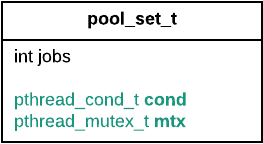
\includegraphics[scale=1]{pool_res.png}
	\label{fig:0}
\end{figure}
\subsection{Concorrenza}
Chiaramente la variabile \textit{jobs} contenuta in \textit{pool\_set\_t} genera una race condition:
\begin{itemize}
\item \textbf{jobs}	letta e scritta da tutti i thread del pool di appartenenza; inizializzata e scritta dal \textit{manager}
\end{itemize} 
Per accedervi è necessario acquisire la \textit{lock} sulla mutex relativa al pool\_set. 
Le variabili di pool nel programma sono 2: una per i cassieri ed una per i clienti. Esse sono scollegate fra loro infatti i cassieri controlleranno solo la loro variabile di pool e viceversa.\\
Il \textit{manager} può modificare \textit{jobs} dei 2 pool nel seguente modo:
\begin{itemize}
\item \textbf{clienti}	ogni E clienti che escono dal supermercato vengono resi disponibili E lavori (\textit{jobs += E})
\item \textbf{casse}	quando riceve la comunicazione dal direttore di aprire una cassa, incrementa di 1 \textit{jobs}
\end{itemize}

\section{Manager}
\subsection{Comunicazione con i Clienti}
Il manager gestisce le comunicazioni dai clienti. Essi comunicano la loro entrata, la loro uscita e l'eventuale richiesta del permesso di uscita nel caso in cui non abbiano effettuato acquisti.\\
Tale comunicazione è gestita con una \textit{unnamed pipe} aperta da entrambe le estremità in ogni thread. 
\subsubsection{Concorrenza}
\begin{itemize}
\item \textbf{pipe, fd[0]} l'unico lettore è il manager, non vi è concorrenza su tale fd
\item \textbf{pipe, fd[1]} possono scrivere sulla pipe tutti i C clienti ed anche il Thread Signal Handler
\end{itemize}
La comunicazione avviene seguendo un protocollo: viene inviato un messaggio di tipo \textit{pipe\_msg\_code\_t} (mostrato in figura \ref{fig:pipemsg})
\begin{figure}[h]
	\centering
	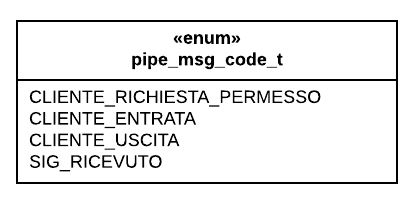
\includegraphics[scale=0.8]{pipemsg.png}
	\caption{pipe\_msg\_code\_t}
	\label{fig:pipemsg}
\end{figure}


\section{Cliente}

\subsection{Concorrenza}
\begin{itemize}
\item elem: \textbf{stato\_attesa}
\item \textbf{permesso\_uscita} scritto solamente dal Manager e letto dal rispettivo cliente; reinizializzato dal cliente\\
=> \hspace{10mm} va acquisita la risorsa attraverso \textit{lock(cond\_cliente)} 

\end{itemize}


\section{Cassiere}

\begin{figure}[h]
	\centering
	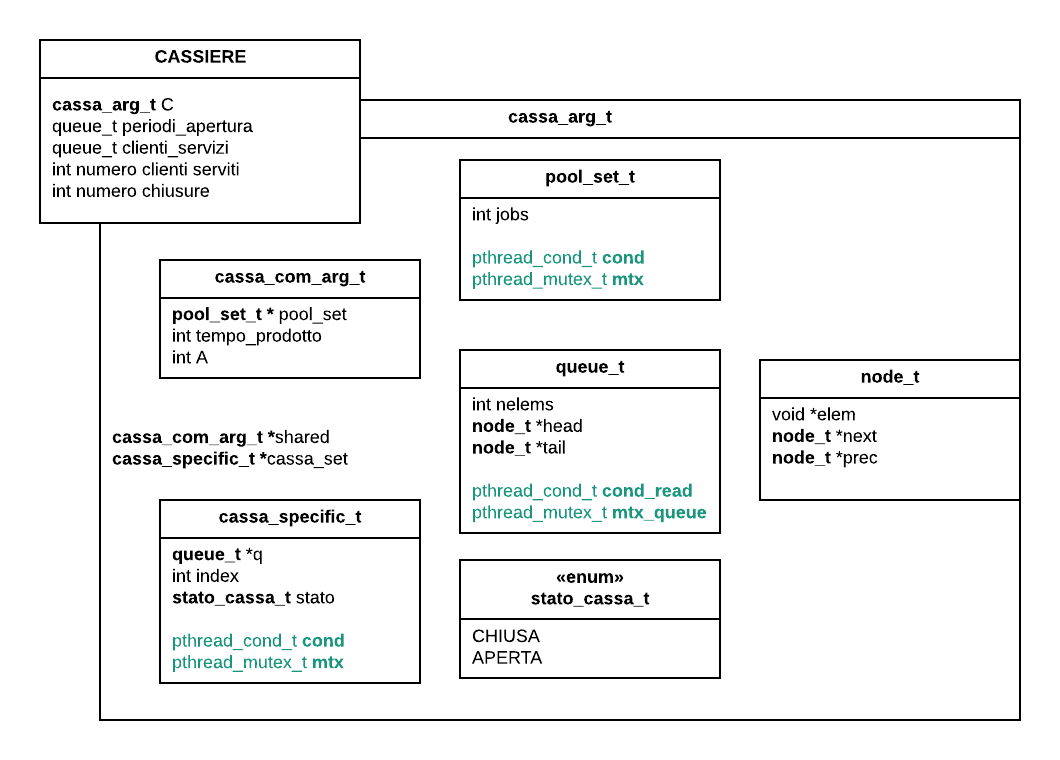
\includegraphics[scale=0.8]{cassa.png}
	\label{fig:cassa}
\end{figure}

\textit{shared} è condiviso fra tutte le casse mentre \textit{cassa\_set} è specifico per ogni cassa
la scelta di  usare un'ulteriore struttura dati è 
per  incapsulamente e riservatezza dei dati 
delle che dovranno essere letti dai clienti 
\subsection{Concorrenza}
Nel cassiere le variabili accedute in lettura e scrittura da più thread sono:
\begin{itemize}
\item q
\item stato
\end{itemize}

\section{Direttore}
\subsection{Comunicazione Direttore-Supermercato}
\section{Utilizzo}

\end{document}